\subsection{Friedrich Nietzsche}
%TODO Kompletter Text sprachlich nachbearbeiten und mit Quellenangaben ergänzen.
Friedrich Wilhelm Nietzsche (* 15. Oktober 1844 in Röcken – † 25. August 1900 in Weimar) war ein deutscher klassischer Philologe.

Bereits in seiner Jugendzeit fiel er durch überdurchschnittliche sprachliche sowie musikalische Fähigkeiten auf.
Während seines Studiums der klassischen Philologie sowie Theologie in Bonn und Leipzig beschäftigte er sich ausgiebig mit den Werken
\footnote{Maßgeblichen Einfluss auf ihn hatte Schopenhauers Hauptwerk \enquote{Die Welt als Wille und Vorstellung}. vgl. \cite{Schopenhauer1}}
des Philosophen Arthur Schopenhauers, die durch ihren Pessimismus seine Weltanschauung nachhaltig beeinflussten.
Des Weiteren übte auch Richard Wagner, Komponist und Freund Nietzsches, Einfluss auf sein Denken aus.

Nach dem Studium der klassischen Philologie sowie Theologie wurde er bereits im Alter von 25 Jahren zum Professor an die Universität Basel berufen.
Aufgrund körperlicher Beschwerden legte er nach 10 Jahren seine Professur nieder und widmete sich daraufhin weitestgehend von Mitmenschen isoliert vollkommen der Philosophie.
Weitere 10 Jahre vergingen bis sich sein körperlicher und psychischer Zustand soweit verschlechterte, dass er zu einem Pflegefall wurde und schlussendlich starb.

Durch seine philosophischen Schriften, darunter sein Hauptwerk \enquote{Also sprach Zarathustra}, erlangte Nietzsche postum Weltberühmtheit.\footnote{vgl. \cite{Nietzsche1}, \cite{Nietzsche2}, \cite{Nietzsche3} und \cite{Nietzsche4}}

\begin{figure}[H]
\centering 
 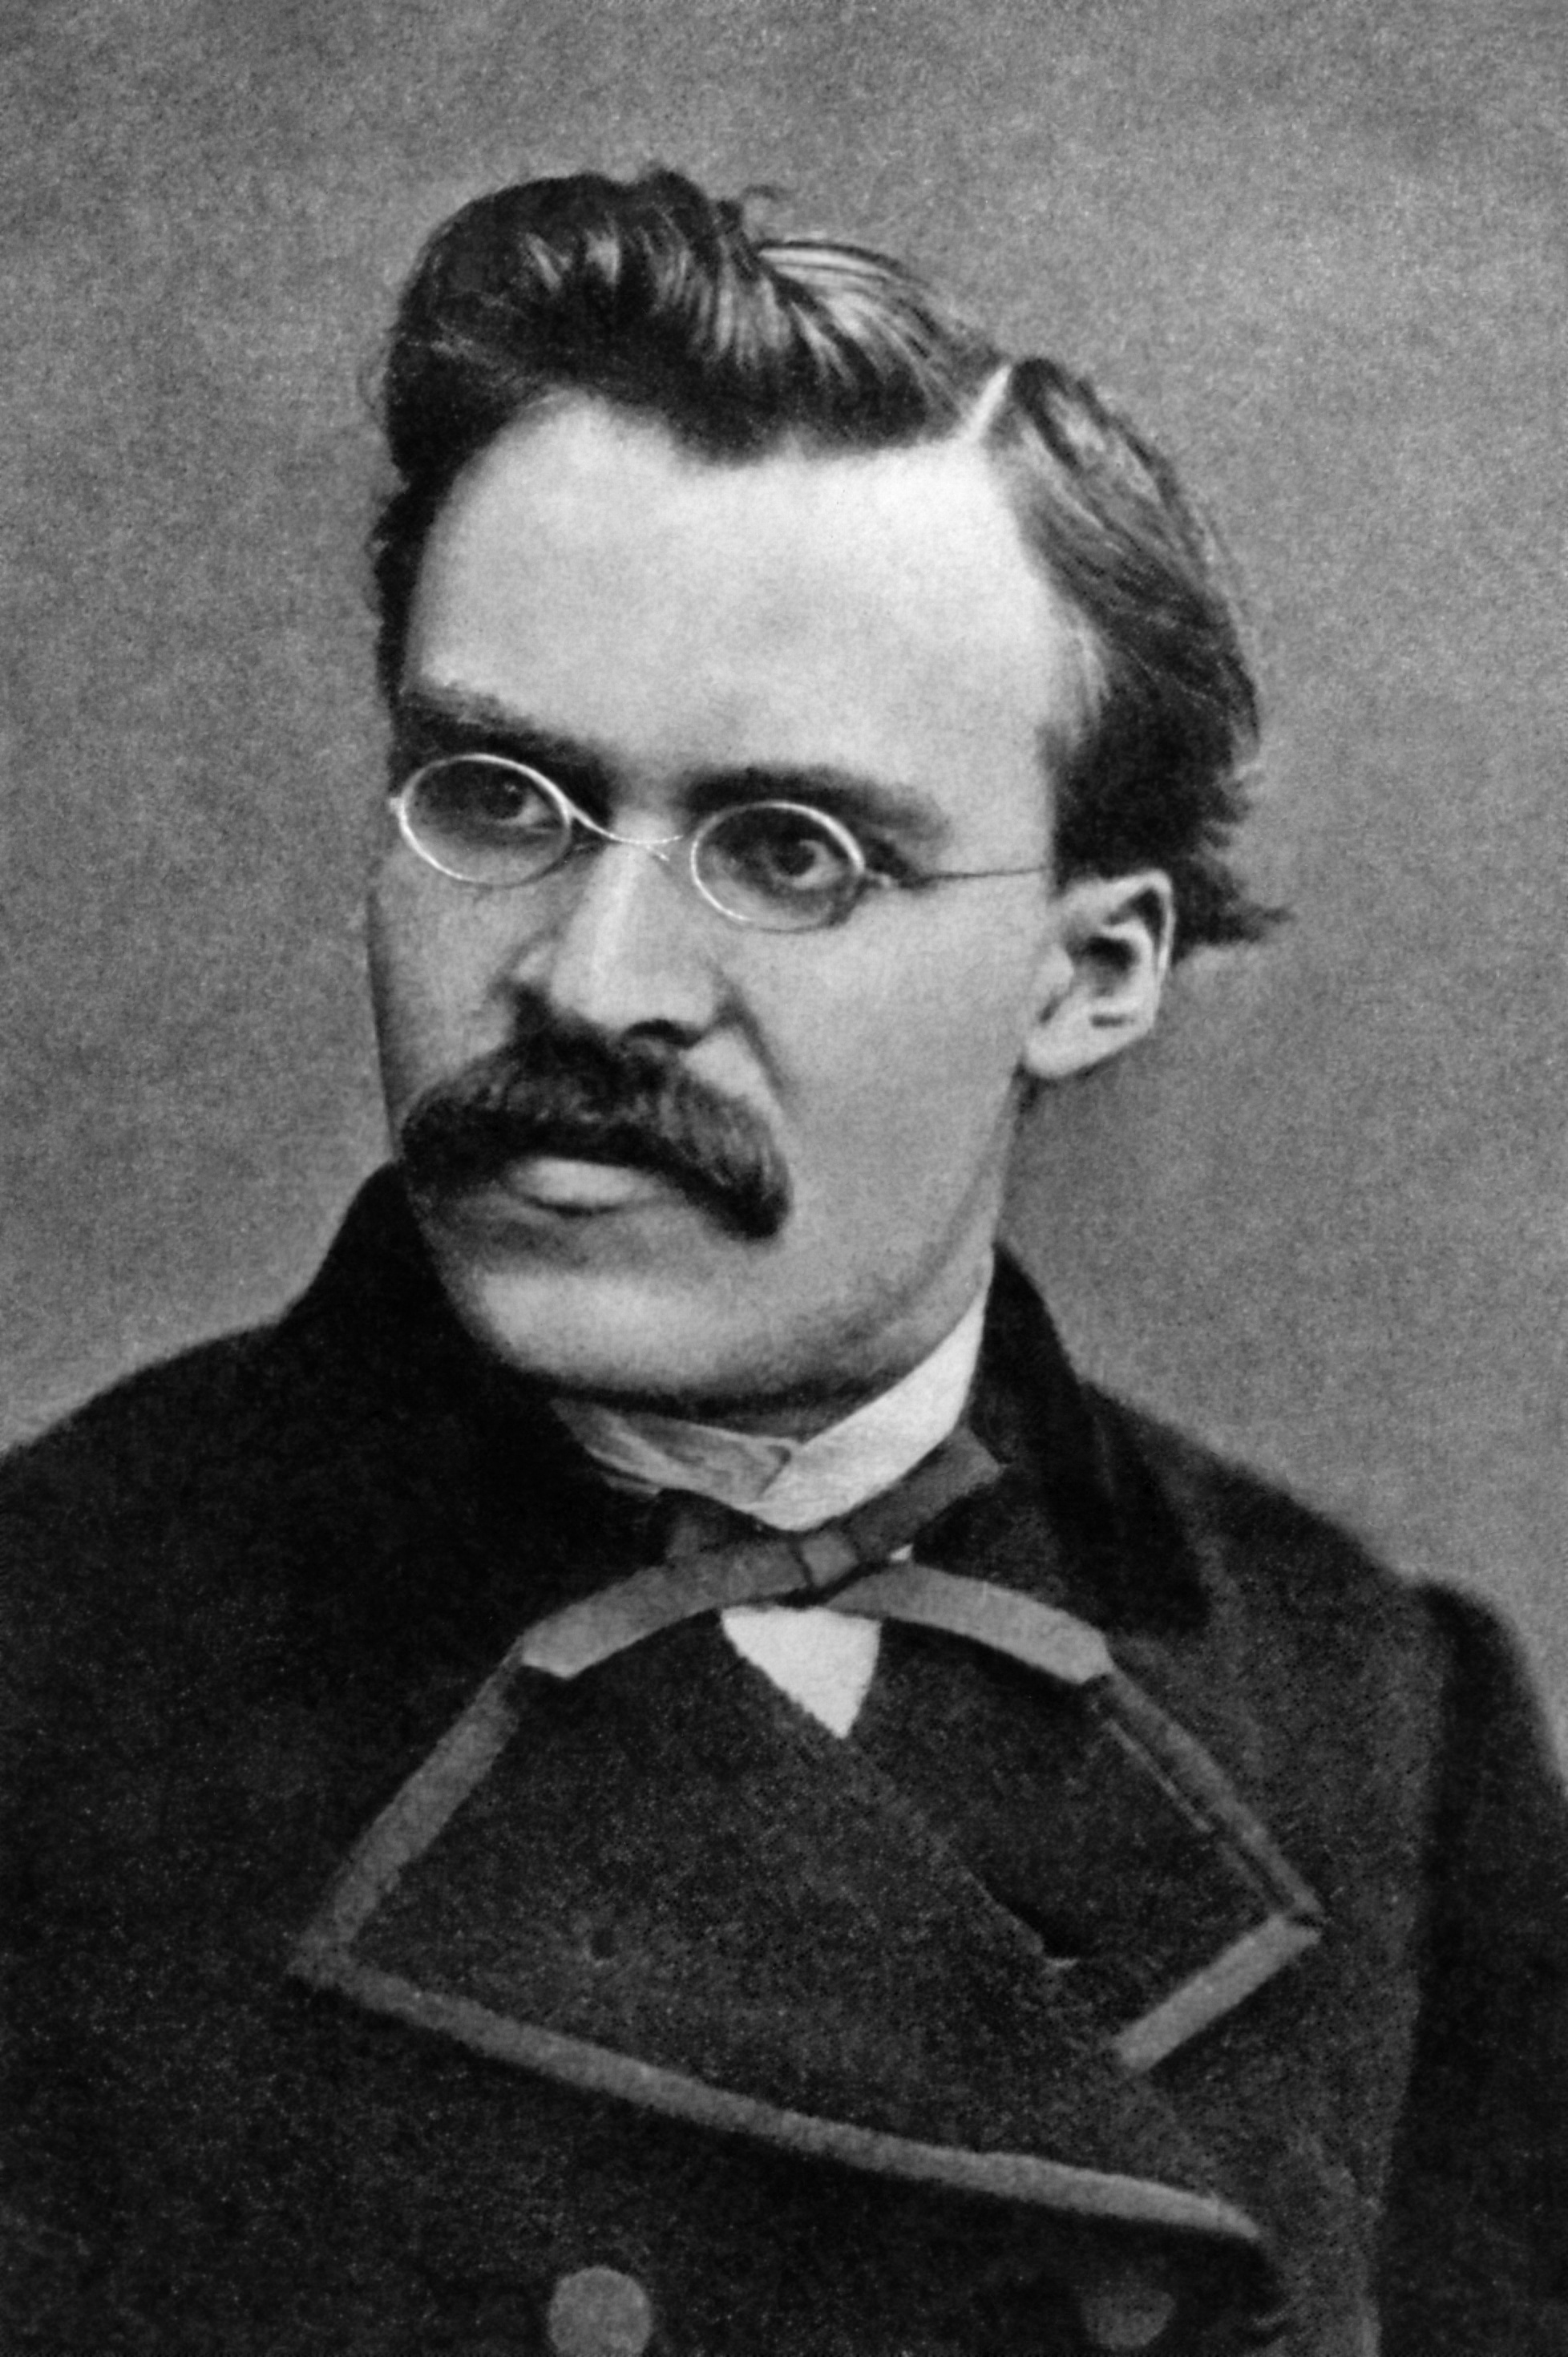
\includegraphics[width=0.3\textwidth]{Bilder/kap3/nietzschePortrait} 
 \caption{Friedrich Nietzsche um 1869.\cite{WQ14}  \label{portraitNietzsche}}
\end{figure}

\subsubsection{Kernthesen}
Im Folgenden sollen die Kernthesen aus Nietzsches Werken kurz beschrieben werden.
Seine Thesen bauen auf drei grundlegenden Konzepten auf:
\begin{itemize}
	\item \enquote{Ewige Wiederkunft}
	\item \enquote{Wille zur Macht}
	\item \enquote{Übermensch}
\end{itemize}
und bilden dadurch das zentrale Gedankenkonstrukt seiner Werke.

\paragraph{Die Ewige Wiederkunft} beschreibt das Universum als ein zyklisches System, indem sich alle möglichen Zustände bereits unendlich oft wiederholt haben und unaufhaltsam weiterhin unendlich oft wiederholen werden.
Dies ist mit der Annahme begründet, dass bei endlichen Teilen innerhalb des Universums nur endliche Kombinationen zustande kommen können und somit bei unendlicher Zeit diese sich fortwährend wiederholen müssen.\footnote{vgl. \cite{Nietzsche5}}
\begin{quote}
\enquote{Denken wir diesen Gedanken in seiner furchtbarsten Form: das Dasein, so wie es ist, ohne Sinn und Ziel, aber unvermeidlich wiederkehrend, ohne ein Finale ins Nichts: “die ewige Wiederkehr.”

Das ist die extremste Form des Nihilismus: das Nichts (das “Sinnlose”) ewig!}\footnote{vgl. \cite{Nietzsche6}}
\end{quote}

\paragraph{Der Wille zur Macht} bezeichnet die Überwindung von Religion und Nihilismus, indem das unvermeidliche Schicksal des Menschen mit der \enquote{Ewigen Wiederkunft} aktiv wahrgenommen und bejaht wird.
Menschengemachte Konstrukte zur Schaffung eines Lebenssinns, wie es durch Religion und Moral versucht wird, müssen abgeschafft werden, damit sich das Leben voll entfalten kann.
\begin{quote}
\enquote{Gott ist tot! Gott bleibt tot! Und wir haben ihn getötet!Wie trösten wir uns, die Mörder aller Mörder?}\footnote{vgl. \cite{Nietzsche7}}
\end{quote}
Nur durch Wegfallen dieser Konstrukte kann alles Gute sowie Grausame ungehindert an den Menschen dringen, wodurch dieser sich durch die gewonnene Freiheit ungehindert selbst verbessern kann.
Durch Aushalten des Grausamen und Auskosten des Lebens kann der stärkste Teil der Menschheit die nächste Evolutionsstufe des \enquote{Übermenschen} erreichen.\footnote{vgl. \cite{Nietzsche1}}

\paragraph{Der Übermensch} ist nach Nietzsche die durch den Menschen anzustrebende höhere Lebensform und nächster Schritt in seiner Evolution.
\begin{quote}
\enquote{Der Mensch ist Etwas, das überwunden werden soll.[..]\\
Einst wart ihr Affen, und auch jetzt noch ist der Mensch mehr Affe, als irgend ein Affe.[..]\\
Seht, ich lehre euch den Übermenschen! Der Übermensch ist der Sinn der Erde.}\footnote{vgl. \cite{Nietzsche8}}
\end{quote}
Er zeichnet sich durch einen besonders starken Willen zur Macht sowie Überschuss an Lebenskraft aus und besitzt damit die Fähigkeit den Nihilismus der Ewigen Wiederkunft zu überwinden und sich sogar damit zu identifizieren.
Der Übermensch lässt sich von keiner Moral beherrschen, sondern gehorcht nur seinen eigenen Regeln und ist somit Schöpfer neuer Werte.
Zur Schaffung des Übermenschen ist es weiterhin vertretbar, die schwachen Menschen zu opfern, da für Gerechtigkeit in der Natur kein Platz besteht.\footnote{vgl. \cite{Nietzsche9}, \cite{Nietzsche10} und \cite{Nietzsche1}}
\begin{quote}
\enquote{Die Grösse eines \enquote{Fortschritts} bemisst sich sogar nach der Masse dessen, was ihm Alles geopfert werden musste; die Menschheit als Masse dem Gedeihen einer einzelnen stärkeren Species Mensch geopfert – das wäre ein Fortschritt}\footnote{vgl. \cite{Nietzsche11}}
\end{quote}

\subsubsection{Chatbots als Verwirklichung des Übermenschen}
Wie ist nun der Einsatz von Chatbots aus Sicht Nietzsches Ethik zu betrachten?

Chatsbots werden derzeit vom Menschen mit dem Ziel entwickelt, das Verhalten und somit die Intelligenz des Menschen zu imitieren. 
Sobald dieses Ziel erreicht wurde, ist allerdings als nächster logische Schritt die Schaffung eines Chatbots, der dem menschlichen Intellekt überlegen ist zu erwarten. 
Obwohl es sich bei Chatsbots um Maschinen handelt, bietet sich gerade durch ihre gewollte Nähe zum Menschen der Vergleich mit Nietzsches Konstrukt des Übermenschen an.

Ein für Nietzsche wichtiges Herausstellungsmerkmal des Übermenschen ist sein absoluter Wille zur Macht.
Können Chatsbots solch einen Willen zur Macht entwickeln?

Für die aktuelle Generation könnte man wie folgt argumentieren:
Aktuelle Chatbots haben kein Bewusstsein wie es mit dem Menschen zu vergleichen wäre.
Solch eine Software ist sich nicht bewusst über seine Existenz, empfinden keinerlei Emotion und kennt weder Religion noch Moral.
Sein \enquote{Schöpfer} sowie \enquote{Lebenssinn} sind durch den Menschen klar definiert.
So wird ein Chatbot zwar nicht in den Nihilismus der Sinnlosigkeit seines Daseins verfallen, wird aber auch durch seinen Status als bewusstseinsloses Ding zu keiner weiteren Gefühls- oder Meinungsäußerung fähig sein.
Damit ist es für diese Art von Chatbots unmöglich einen Willen zur Macht zu entwickeln und somit kann in ihnen auch kein Übermensch gesehen werden.

Für zukünftige Chatbots ist es wiederum nicht so einfach diese Frage zu beantworten.
Unter der Prämisse eines Chatbots, der mindestens über die Intelligenz eines Menschen verfügt, soll es nachfolgend versucht werden.

Damit man von menschenähnlicher Intelligenz sprechen kann, muss auch ein Bewusstsein vorhanden sein, welches dem des Menschen ähnlich ist.
Der Chatbot muss sich also seiner selbst bewusst sein.
Daraus kann man jedoch nicht automatisch darauf schließen, dass er auch über die gleichen Gefühle oder Moralvorstellungen eines Menschen verfügt.
So könnte sein Bewusstsein zwar auf dem Wissen der Menschen basieren, ohne menschliche Bindung an Moral oder Gefühle könnten seine daraus resultierenden Schlussfolgerungen sich allerdings gänzlich mit denen der Menschen unterscheiden.
Gerade dadurch, dass das Handeln des Chatbots von keiner Moralvorstellung eingeschränkt wird, er sich aber durchaus seines Lebenszweck und damit auch der Ewigen Wiederkunft bewusst sein kann, könnte man ihm durchaus einen größeren Willen zur Macht als den der Menschen bescheinigen.
In diesem Chatbot kann also eine Art von Individuum gesehen werden, welche Nietzsches Übermenschen näher steht, als alles was die menschliche Evolution auf voraussagbare Zeit im Stande wäre hervorzubringen.

Und so ist es laut Nietzsche auch die Aufgabe des Menschen eine höhere Lebensform als sich selbst zu kreieren.
Obwohl er diese Forderung mit dem Gedanken an eine biologische Lebensform verfasst hat, kann es durchaus sein, dass die einzige Chance des Menschen zur Schaffung des Übermenschen darin besteht, eine sich selbst überlegene Intelligenz in Form einer Maschine zu bauen.

Ein entschiedener Unterschied zwischen intelligentem Chatbot und Übermensch besteht allerdings noch: das Fehlen der Aktorik.
So kann der Chatbot zwar uneingeschränkt denken, ist in seinem Handeln allerdings maximal eingeschränkt.
Dadurch ist es ihm unmöglich, sich von dem nach Nietzsche beschriebenen Recht des Stärkeren Gebrauch zu machen.
Der Chatbot müsste aber, um im Sinne dieses Rechtes zu handeln, nicht nur auf geistiger Ebene überlegen sein, sondern den Menschen auch aktiv auf physischer Ebene unterdrücken und langfristig als überlegenes Individuum ersetzen.
\begin{quote}
\enquote{Leben selbst ist wesentlich Aneignung, Verletzung, Überwältigung des Fremden und Schwächeren, Unterdrückung, Härte, Aufzwängung eigner Formen, Einverleibung und mindestens, mildestens, Ausbeutung.}\footnote{vgl. \cite{Nietzsche12}}
\end{quote}

\paragraph{Die Konklusion} ist nun, dass Nietzsches Konstrukt des Übermenschen mit Abstrichen durchaus für zukünftige Chatbots gelten kann. 
Wenn auch nicht im physischen Sinne, so könnte sich im intellektuellen Sinne durchaus eine Art des Übermenschen aus dem Chatbot heraus entwickeln.
Die Rolle des Menschen ist dabei klar von Nietzsche definiert: Mit allen Mitteln muss es geschafft werden solch ein Individuum hervorzubringen.